\documentclass[9pt,pdftex,xcolor=dvipsnames]{beamer}
\setbeamertemplate{section in toc}[sections numbered]
\setbeamertemplate{subsection in toc}%
{\leavevmode\leftskip=3em\rlap{\hskip-2em\inserttocsectionnumber.\inserttocsubsectionnumber}\inserttocsubsection\par}
% use git: import repository as new project in eclipse: http://www.eclipse.org/forums/index.php/t/226301/
\usepackage[utf8]{inputenc}
\usepackage[english]{babel}
\usepackage{amsfonts, amsmath, amssymb}
\usepackage[bf,small, format=plain]{caption}
\usepackage{color}
\usepackage{bbding}
\usepackage{bm} %bold math

%\usepackage[usenames,dvipsnames]{xcolor}
\usepackage{graphicx}
\usepackage{tikz,tikzscale,pgfplots,grffile}
\usetikzlibrary{arrows,shapes,backgrounds}
\usetikzlibrary{plotmarks}
\usepackage{bbding}

\usepackage[clock]{ifsym}

\usepackage{pgfplots}
\usepackage{grffile}
\pgfplotsset{compat=newest}

%\author{}
%\title{}
%\setbeamercovered{transparent} 
%\setbeamertemplate{navigation symbols}{} 
%\logo{} 
%\institute{} 
%\date{} 
%\subject{} 

\pgfdeclarelayer{bg}
\pgfsetlayers{bg,main}

\definecolor{grey}{rgb}{0.9,0.9,0.9}
\usepackage{listings}
\lstset{language=C++,
				breaklines=true,
				tabsize=8,
				showtabs=true,
                basicstyle=\scriptsize\ttfamily,
                keywordstyle=\color{blue}\ttfamily,
                stringstyle=\color{red}\ttfamily,
                commentstyle=\color{OliveGreen}\ttfamily,
                morecomment=[l][\color{magenta}]{\#},
                frame = single,
                backgroundcolor=\color{grey} 
}
\usepackage{mdframed}
\usepackage{multicol}
\usepackage{tcolorbox}
%\usepackage{multirow}
% \usepackage{paralist}
%\usepackage[colorinlistoftodos]{todonotes}
%\usepackage{biblatex}
%usepackage[nolist,nohyperlinks]{acronym}
%\usepackage{amstext}
%\usepackage{hyperref} 
%\usepackage{comment}
%\usepackage{subcaption}
%\renewcommand*{\figureautorefname}{fig.}
%\renewcommand*{\equationautorefname}{eq.}
\usepackage{bm}
\usepackage{comment}
%\usepackage{beamerthemeshadow}
%\usepackage{tikz}
%\usepackage{pgfplots}
%\usepackage{ulem}
%\usepackage[lofdepth,lotdepth]{subfig}
%\newenvironment{figure*}%
%{\begin{figure}}
%{\end{figure}}
%\usepackage[style=mla,babel=hyphen,backend=biber]{biblatex}
% CSE-Beamer-Styles:
\usepackage[course]{beamertheme_sccstalk}
%\usepackage[lecture]{beamertheme_sccstalk}
\usepackage{beamercolorscheme_sccs}
\usepackage{beamerfontthemestructurebold}
\setcounter{tocdepth}{3} 
%colored blocks, example \begin{variableblock}{Title}{bg=blue,fg=white}{bg=white,fg=black}
\newenvironment{variableblock}[4]{%
\setbeamercolor{block title}{#2}
\setbeamercolor{block body}{#3}
\begin{block}{#1}\begin{mdframed}{#4}\end{mdframed}\end{block}}


%some useful commands
%\newcommand{\der}[2]{\frac{\text{d}#1}{\text{d}#2}}
\title{Assignment 4: MPI Collectives and MPI-IO}
\subtitle{Programming of Super Computers}
\author[Friedrich Menhorn, Benjamin Rüth, Erik Wannerberg] {Friedrich Menhorn, Benjamin Rüth, Erik Wannerberg \\ Team 12} %[displayed in footer]{displayed on title page}
\date{\today}
\institute{Technische Universität München}
\newtheorem*{rem}{Remark}

\usepackage[backend=biber]{biblatex}
\bibliography{References/refs}

\begin{document}
\frame{\maketitle}

\begin{frame}{Contents}
\tableofcontents
\end{frame}


\section{MPI Collectives}
\begin{frame}{\phantom{Contents}}
\tableofcontents[
  currentsection  
]
\end{frame}


\subsection{Optimizations}
\begin{frame}[fragile]{\insertsubsection}
Sending the dimensions of the matrix to all processes:
\begin{columns}
\column[t]{.5\textwidth}
\begin{block}{Original code:}
\begin{lstlisting}
// send dimensions to all peers
if(rank == 0) {
    int i;
    for(i = 1; i < size; i++){
        MPI_Send(matrices_a_b_dimensions, 4, MPI_INT, i, 0, cartesian_grid_communicator);
    }
} else {
    MPI_Recv(matrices_a_b_dimensions, 4, MPI_INT, 0, 0, cartesian_grid_communicator, &status);
}
\end{lstlisting}
\end{block}

\column[t]{.5\textwidth}
\begin{block}{With collective operation:}
\begin{lstlisting}	
// send dimensions to all peers
MPI_Bcast(matrices_a_b_dimensions, 4, MPI_INT, 0, cartesian_grid_communicator);
\end{lstlisting}
\end{block}
\end{columns}
\end{frame}

\begin{frame}[fragile]{\insertsubsection \ (contd.)}
Distribute matrix blocks among all processes:
\begin{columns}
\column[t]{.5\textwidth}
\begin{block}{Original code:}
\begin{lstlisting}
// send a block to each process
if(rank == 0) {
    int i;
    for(i = 1; i < size; i++){
        MPI_Send(A_array, ...);
        MPI_Send(B_array, ...);
    }
    for(i = 0; i < A_local_block_size; i++){
        A_local_block[i] = A_array[i];
    }
    for(i = 0; i < B_local_block_size; i++){
        B_local_block[i] = B_array[i];
    }
} else {
    MPI_Recv(A_local_block, ...);
    MPI_Recv(B_local_block, ...);
}
\end{lstlisting}
\end{block}

\column[t]{.5\textwidth}
\begin{block}{With collective operation:}
\begin{lstlisting}	
// send a block to each process
MPI_Scatter(A_array, A_local_block_size, MPI_DOUBLE, A_local_block, A_local_block_size, MPI_DOUBLE, 0, cartesian_grid_communicator);
MPI_Scatter(B_array, B_local_block_size, MPI_DOUBLE, B_local_block, B_local_block_size, MPI_DOUBLE, 0, cartesian_grid_communicator);
\end{lstlisting}
\end{block}
\end{columns}
\end{frame}

\begin{frame}[fragile]{\insertsubsection \ (contd.)}
Distribute matrix blocks among all processes and do initial rotation of blocks:
\begin{columns}
\column[t]{.5\textwidth}
\begin{block}{Original code:}
\begin{lstlisting}
// send a block to each process
...
// fix initial arrangements before the core algorithm starts
if(coordinates[0] != 0){
    MPI_Sendrecv_replace(A_local_block, ...);
}
if(coordinates[1] != 0){
    MPI_Sendrecv_replace(B_local_block, ...);
}
\end{lstlisting}
\end{block}

\column[t]{.5\textwidth}
\begin{block}{With collective operation:}
\begin{lstlisting}	
// send a block to each process and fix initial arrangements before the core algorithm starts
int *send_count= (int *) malloc(...);
int *displs_A = (int *) malloc(...);
int *displs_B = (int *) malloc(...);
int displ_coord_A_col = ... 
int displ_coord_B_row = ...
int displs_local_A = ...
int displs_local_B = ...

MPI_Gather(&displs_local_A, ...);
MPI_Gather(&displs_local_B, ...);  
  
for(i = 0; i < size; i++){
	send_count[i] = A_local_block_size;
}

MPI_Scatterv(A_array, ...);
MPI_Scatterv(B_array, ...);
\end{lstlisting}
\end{block}
\end{columns}
\end{frame}


\begin{frame}[fragile]{\insertsubsection \ (contd.)}
Collect results after computation loop:
\begin{columns}
\column[t]{.5\textwidth}
\begin{block}{Original code:}
\begin{lstlisting}
// get C parts from other processes at rank 0
if(rank == 0) {
    for(i = 0; i < A_local_block_rows * B_local_block_columns; i++){
        C_array[i] = C_local_block[i];
    }
    int i;
    for(i = 1; i < size; i++){
        MPI_Recv(....);
    }
} else {
    MPI_Send(...);
}
\end{lstlisting}
\end{block}

\column[t]{.5\textwidth}
\begin{block}{With collective operation:}
\begin{lstlisting}	
// get C parts from other processes at rank 0
int C_local_block_size = A_local_block_size;
	MPI_Gather(C_local_block, C_local_block_size, MPI_DOUBLE, C_array, C_local_block_size, MPI_DOUBLE, 0, cartesian_grid_communicator);
\end{lstlisting}
\end{block}
\end{columns}
\end{frame}
	


\begin{frame}{\insertsubsection \ (contd.)}
\begin{block}{Expectations}
\begin{itemize}
\item \textbf{Performance:\\}
Higher performance due to highly optimized MPI collectives (might also consider network topology etc.) vs. naive implementation via \lstinline[basicstyle=\ttfamily]{MPI_Send/MPI_Recv}.

\item \textbf{Scaling:\\}
Efficient implementation of Broadcast, Gather, Scatter use treelike distribution of values, $\mathcal{O}\left(n\right) \rightarrow \mathcal{O}\left(\log(n)\right)$. This means we also benefit with respect to scalability.
\end{itemize}
\end{block}
\end{frame}


\begin{frame}{\insertsubsection \ (contd.)}
\begin{block}{Readability and Maintainability}
\begin{itemize}
\item[\textcolor{YellowGreen}{$\bm\oplus$}] Sending dimensions with \lstinline[basicstyle=\ttfamily]{MPI_Bcast}
\item[\textcolor{YellowGreen}{$\bm\oplus$}] Distributing matrix blocks \lstinline[basicstyle=\ttfamily]{MPI_Scatter}
\item[\textcolor{red}{$\bm\ominus$}]
Distributing matrix blocks and initial alignment with \lstinline[basicstyle=\ttfamily]{MPI_Scatterv} 
	\begin{itemize}
	\item[$\rightarrow$] introduces complicated offsets 
	\item[$\rightarrow$] hard to see what actually happens (distribution \& rotation)
	\end{itemize} 
\item[\textcolor{YellowGreen}{$\bm{\oplus}$}] Collecting results using \lstinline[basicstyle=\ttfamily]{MPI_Gather}
\end{itemize}
\end{block}
\end{frame}



\subsection{Performance Measurements}
\begin{frame}{\insertsubsection}
\begin{minipage}{0.45\textwidth}
\begin{figure}
\centering
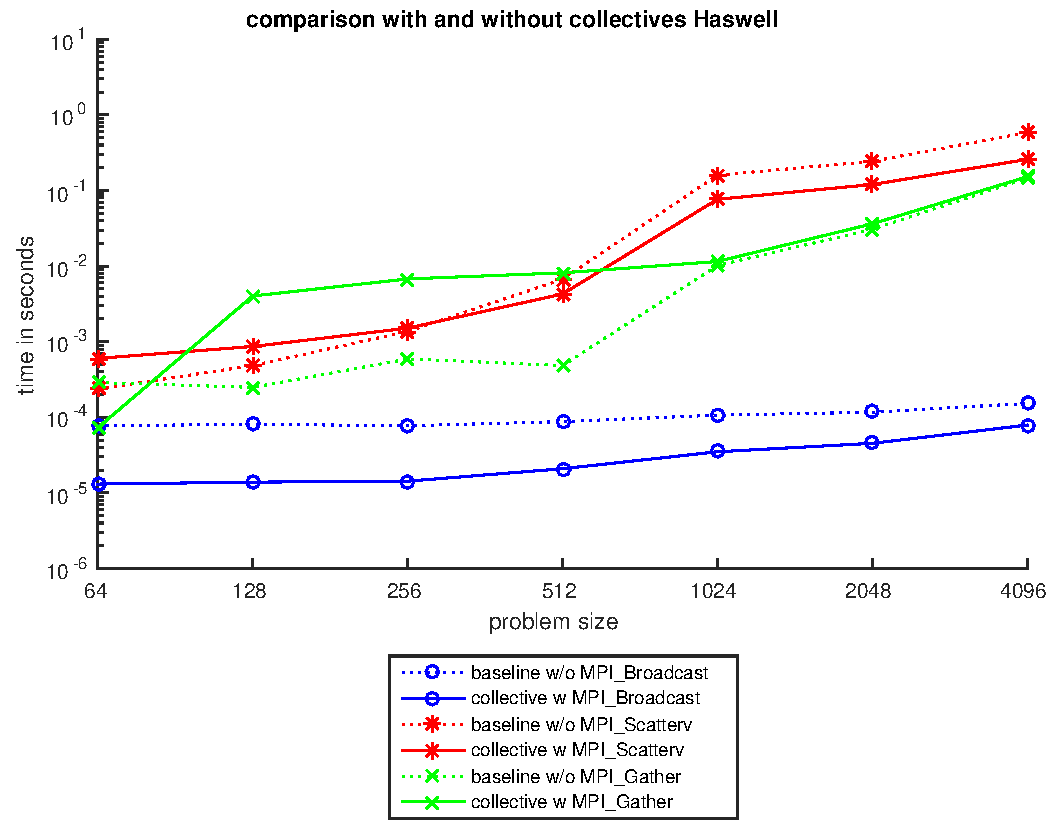
\includegraphics[scale=0.3]{img/comparison_hw_collectives.pdf}
\end{figure}
\end{minipage}
\hspace{0.2cm}
\begin{minipage}{0.45\textwidth}
\begin{figure}
\centering
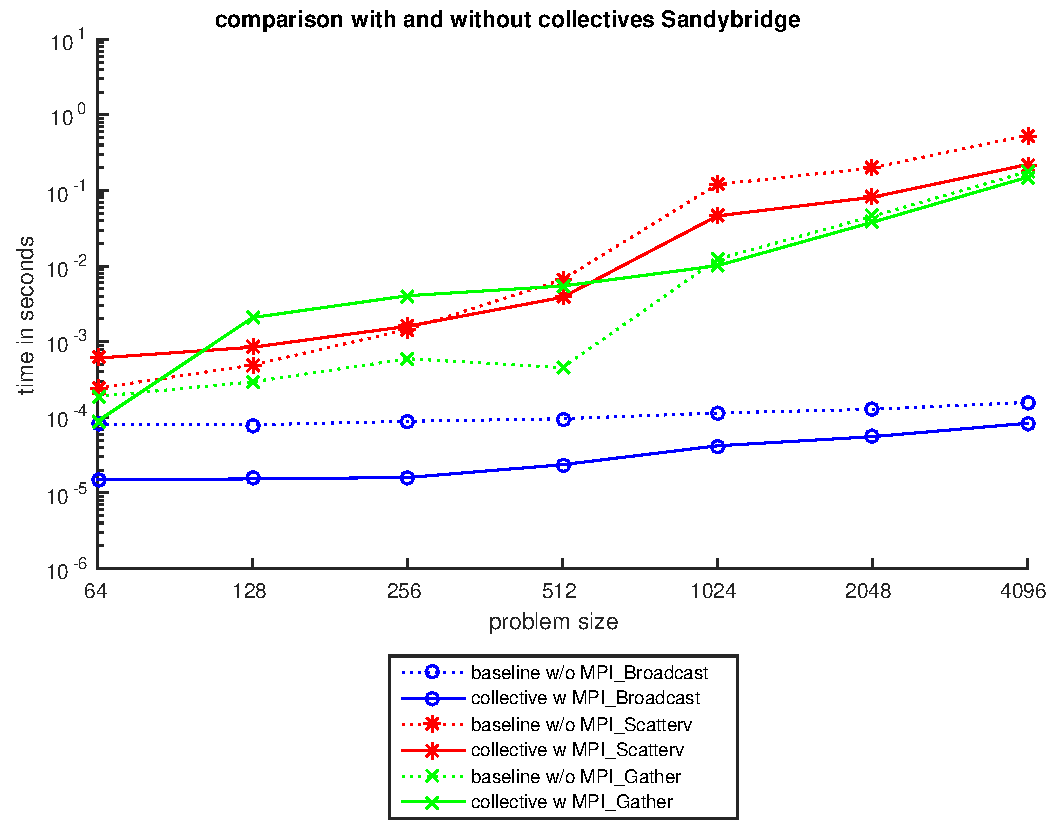
\includegraphics[scale=0.3]{img/comparison_sb_collectives.pdf}
\end{figure}
\end{minipage}
\end{frame}


\section{MPI Parallel IO}
\begin{frame}{\phantom{Contents}}
\tableofcontents[
  currentsection  
]
\end{frame}


\subsection{Data Sieving and 2-Phase IO}
\begin{frame}{\insertsubsection}
What is "Data Sieving" and "2-Phase IO"? How do they help improve IO performance?
\end{frame}

\begin{frame}{Data Sieving}
\begin{itemize}
	\item Read/write larger chunks from files to get fewer system IO calls
	\item "Sieve out" the requested data from the data in-between
	\item More data transferred, especially for writing, and requires buffer -- therefore needs tuning
	\item Controllable by setting an MPI\_Info object with "\texttt{romio\_ds\_reading}" and "\texttt{romio\_ds\_writing}" to "\texttt{enable}" -- other tuning flags available
\end{itemize}
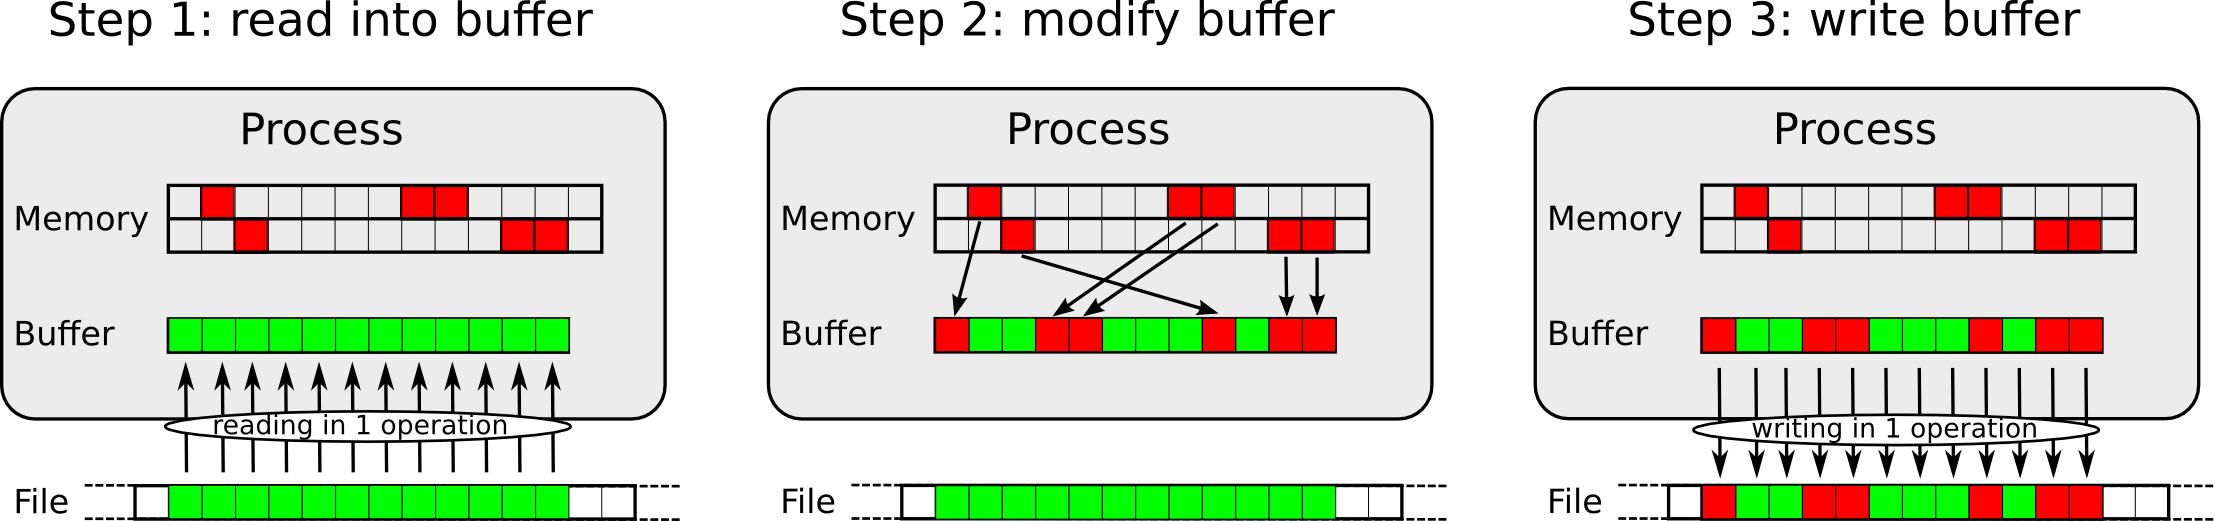
\includegraphics[width=\textwidth]{img/datasieving.png}
\end{frame}

\begin{frame}{2-phase IO}
\begin{itemize}
	\item Same idea as data sieving -- let fewer processes read larger contigous chunks
	\item Distribute data to the requesting processes from buffers via scatters
	\item Controllable by setting an MPI\_Info object with "\texttt{romio\_cb\_reading}" and "\texttt{romio\_cb\_writing}" to "\texttt{enable}" -- other tuning flags available
\end{itemize}
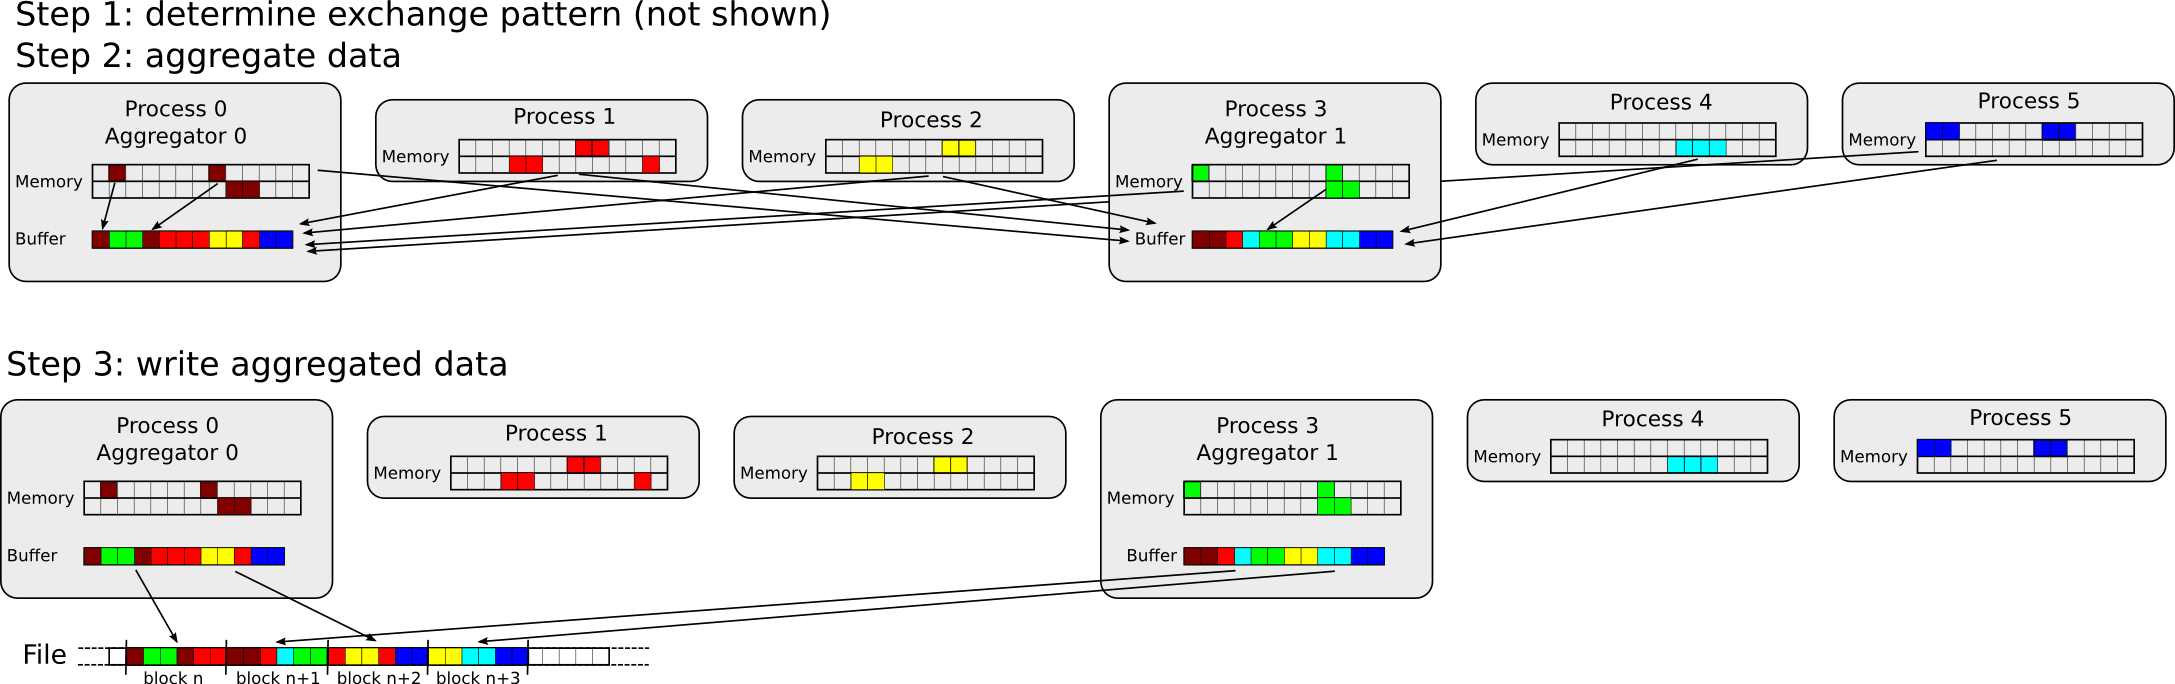
\includegraphics[width=\textwidth]{img/2phaseio.png}
\end{frame}

\subsection{Scalability of original application}
\begin{frame}{\insertsubsection}
\begin{itemize}
\item Was the original implementation scalable in terms of IO performance?
\item Was the original implementation scalable in terms of RAM storage?
\end{itemize}
\end{frame}

\defverbatim[colored]\ioBaselineCodeRead{%
\begin{lstlisting}[basicstyle=\tiny\ttfamily]
if (rank == 0){
   int row, column;
   if ((fp = fopen (argv[1], "r")) != NULL){
       fscanf(fp, "%d %d\n", &matrices_a_b_dimensions[0], &matrices_a_b_dimensions[1]);
       A = (double **) malloc (matrices_a_b_dimensions[0] * sizeof(double *));
       for (row = 0; row < matrices_a_b_dimensions[0]; row++){
            A[row] = (double *) malloc(matrices_a_b_dimensions[1] * sizeof(double));
            for (column = 0; column < matrices_a_b_dimensions[1]; column++)
                fscanf(fp, "%lf", &A[row][column]);
        }
        fclose(fp);
    } else {
        if(rank == 0) fprintf(stderr, "error opening file for matrix A (%s)\n", argv[1]);
        MPI_Abort(MPI_COMM_WORLD, -1);
    }
    /* Here same for B matrix */

    // need to check that the multiplication is possible given dimensions 
    /* Checks for right dimensions */
}
\end{lstlisting}}%

\defverbatim[colored]\ioMPICodeRead{%
\begin{lstlisting}[basicstyle=\tiny\ttfamily]
MPI_Info readInfo;
MPI_Info_create(&readInfo);
int ierr;
int blocksize_A[2] = {A_rows, A_columns*characters_per_number};
MPI_Datatype datatype_blocks_A;
int subsize_A[2] = {A_local_block_rows, A_local_block_columns*characters_per_number};
int array_of_starts_A[2] = {coordinates[0]*A_local_block_rows,((coordinates[1] + coordinates[0]) % sqrt_size)*A_local_block_columns*characters_per_number};    //This shifts the starting coordinate according to the original shift in Cannon's algorithm!
ierr = MPI_Type_create_subarray(2, blocksize_A, subsize_A, array_of_starts_A, MPI_ORDER_C, MPI_CHAR, &datatype_blocks_A);          
MPI_Type_commit(&datatype_blocks_A);
MPI_File mpi_file_matrixA;
ierr=MPI_File_open(MPI_COMM_WORLD, argv[1], MPI_MODE_RDONLY | MPI_MODE_UNIQUE_OPEN, MPI_INFO_NULL, &mpi_file_matrixA);
if (ierr!=MPI_SUCCESS) {printf(" Cannot open file\n");}
MPI_File_set_view(mpi_file_matrixA, A_file_header_size, MPI_CHAR, datatype_blocks_A, "native", readInfo);
	
MPI_File_read_all(mpi_file_matrixA, A_local_block_read, A_local_block_size * characters_per_number, MPI_CHAR, MPI_STATUS_IGNORE);
		
MPI_File_close(&mpi_file_matrixA);
\end{lstlisting}}%

\defverbatim[colored]\ioMPICodeWrite{%
\begin{lstlisting}[basicstyle=\tiny\ttfamily]
int blocksize_C[2] = {A_rows, B_columns};
MPI_Datatype datatype_blocks_C;
int subsize_C[2] = {A_local_block_rows, B_local_block_columns};
int array_of_starts_C[2] = {coordinates[0]*A_local_block_rows, coordinates[1]*B_local_block_columns};    //This shifts the starting coordinate according to the original shift in Cannon's algorithm!
                           
ierr = MPI_Type_create_subarray(2, blocksize_C, subsize_C, array_of_starts_C, MPI_ORDER_C, MPI_DOUBLE, &datatype_blocks_C);
	
MPI_Type_commit(&datatype_blocks_C);
MPI_File mpi_file_matrixC;
ierr=MPI_File_open(MPI_COMM_WORLD, output_filename, MPI_MODE_WRONLY | MPI_MODE_CREATE | MPI_MODE_UNIQUE_OPEN, MPI_INFO_NULL, &mpi_file_matrixC);
if (ierr!=MPI_SUCCESS) {printf(" Cannot open file\n");} 
MPI_File_set_view(mpi_file_matrixC, 0, MPI_DOUBLE, datatype_blocks_C, "native", writeInfo);
	
MPI_File_write_all(mpi_file_matrixC, C_local_block, C_local_block_size, MPI_DOUBLE, MPI_STATUS_IGNORE);
		
MPI_File_close(&mpi_file_matrixC);
\end{lstlisting}}%
\subsection{Impact of parallel IO}

\subsubsection{Reading Data}
\begin{frame}[fragile]{\insertsubsection--\insertsubsubsection}
\begin{overlayarea}{\textheight}{\textwidth}
How much of the communication in the application was replaced with MPI-IO operations? \\
\only<1>{
\begin{block}{Original code (line 55-106):}
\ioBaselineCodeRead
\end{block}
}
\only<2>{
\begin{block}{Using MPI IO:}
\ioMPICodeRead
\end{block}
}
\end{overlayarea}
\end{frame}

\subsubsection{Writing Data}
\begin{frame}[fragile]{\insertsubsection--\insertsubsubsection}
\begin{overlayarea}{\textheight}{\textwidth}
How much of the communication in the application was replaced with MPI-IO operations? \\
\begin{block}{MPI Code (line 55-106):}
\ioMPICodeWrite
\end{block}
\end{overlayarea}
\end{frame}

\subsection{Performance Measurements}
\begin{frame}{\insertsubsection}
\only<1>{
Total IO time = read (+ scatter) (+ gather) + write \\
\begin{figure}
\centering
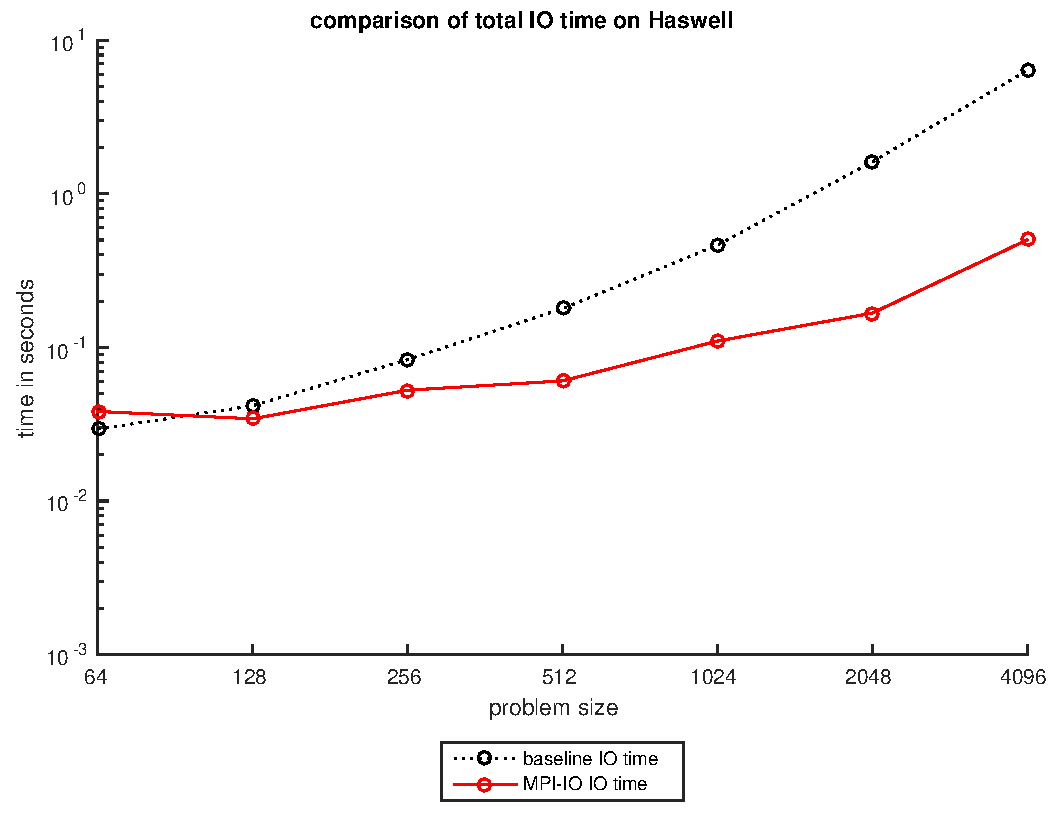
\includegraphics[scale=0.3]{img/comparison_hw_io_all.pdf}
\end{figure}
}
\only<2>{
Setup time = read (+ scatter) \\
Teardown time = write (+ gather) \\
\begin{minipage}{0.45\textwidth}
\begin{figure}
\centering
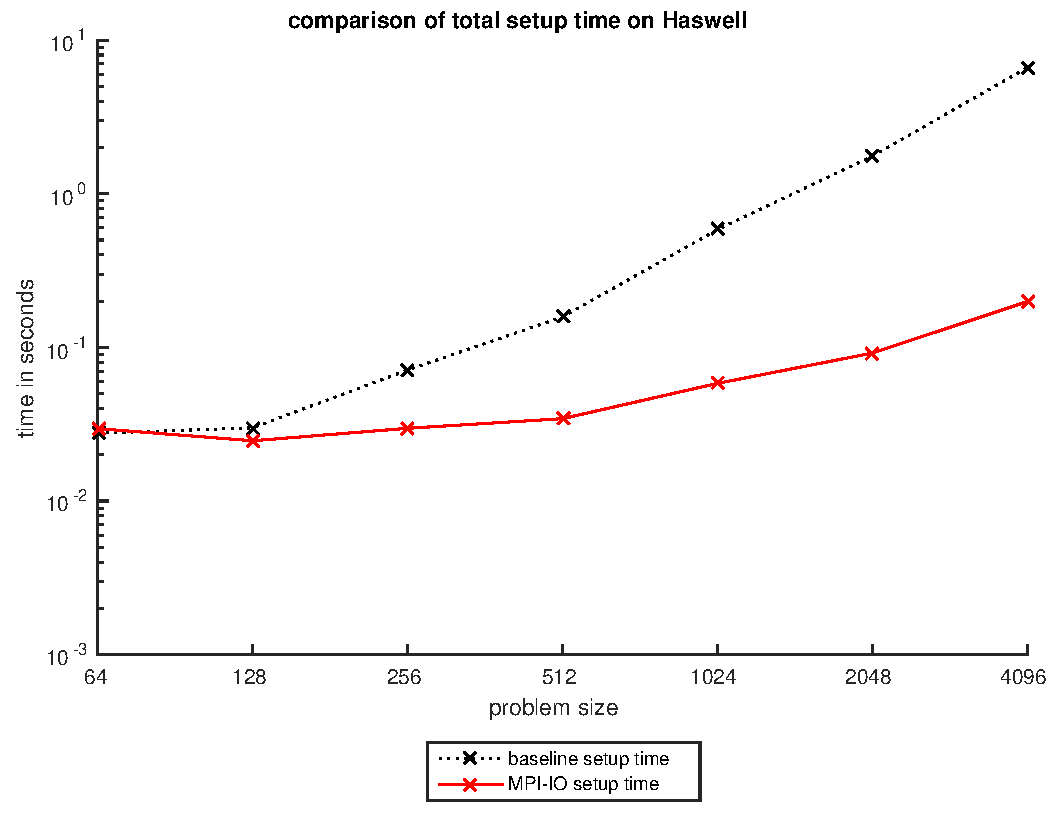
\includegraphics[scale=0.3]{img/comparison_hw_io_su.pdf}
\end{figure}
\end{minipage}
\hspace{0.2cm}
\begin{minipage}{0.45\textwidth}
\begin{figure}
\centering
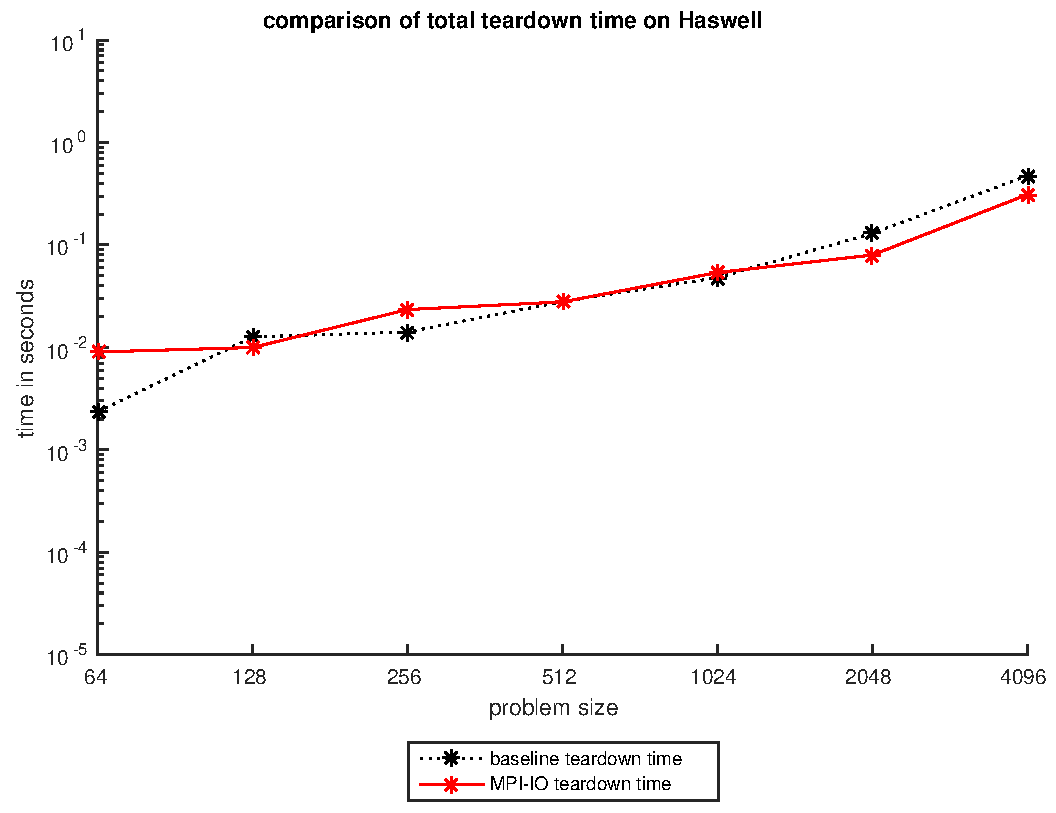
\includegraphics[scale=0.3]{img/comparison_hw_io_td.pdf}
\end{figure}
\end{minipage}
}
\end{frame}


\end{document}